\section{Tests and Results}

\subsection{Instances}
	The instances chosen are taken from the exercises done in laboratory, from a Random Generator\footnote{An update version of the matrix generation of my colleague Federico Ghirardelli.} of symmetric matrices with board size of 50x50 and by a Random Area Generator. 
	
	
	\paragraph{Random Area Generator} This generator builds a symmetric matrix that try to represent a real PCB instance. In fact a real PCB instance contains some patterns. I individualized two of this patterns: square frame of points and order lines of points. Furthermore there are some random points that have a linear disposition in a random position, it can also be inside an area. 
	
	The generator builds an instance with:
	\begin{itemize}
		\item 3 square frame that have the following characteristics:
			\begin{itemize}
				\item random width and height;
				\item random position in a 50x50 board;
				\item not overlap with others areas;
				\item a random number of points:
				\begin{equation*}
					\frac{P_{tot}}{20} \leq P_{area} \leq \frac{P_{tot}}{5}  
				\end{equation*}
				\item the points inside form a square shape and have equal distance;
			\end{itemize}
		\item 4 lines that have the following characteristics:
			\begin{itemize}
				\item $Height = P_{tot} / 20$;
				\item random position in a 50x50 board;
				\item a random number of points: $3 \leq P_{line} \leq 8$;
				\item constant distance between points.
			\end{itemize}
	\end{itemize}

	The figures~\ref{fig:fakeBoards} show the \verb|fb60| instance and the \verb|fb100| instance used.
	
\newpage
	\paragraph{Instances files}
	The pattern use for naming the file is:
	\begin{center}
		\verb|<group><N>.dat|
	\end{center}
	Where \verb|N| is the number of nodes and \verb|group| meaning the origin of that instances.
	
	The instances chosen are (\verb|.dat| is omitted):
	\begin{itemize}
		\item \verb|tsp12|
		\item \verb|tsp60|
		\item \verb|rnd60|
		\item \verb|fb60|
		\item \verb|rnd80|
		\item \verb|fb80|
		\item \verb|rnd100|
		\item \verb|rnd100_2|: build with random generator but with board size 60x60;
		\item \verb|fb100|
	\end{itemize}
	I prefer to select instance with an equal number of nodes but made from different source in order to see how much the instance form impact on the results of meta heuristic methods.
	
	After done this step I took real instances from PCB projects that I will explain in next section \ref{sec:realDomainTests}. 

	\begin{figure}[hb]
		\centering
		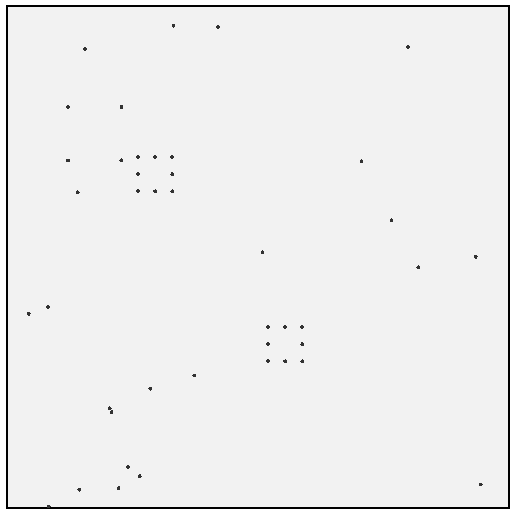
\includegraphics[width=0.44\textwidth]{img/fb60}%
		\qquad\qquad
		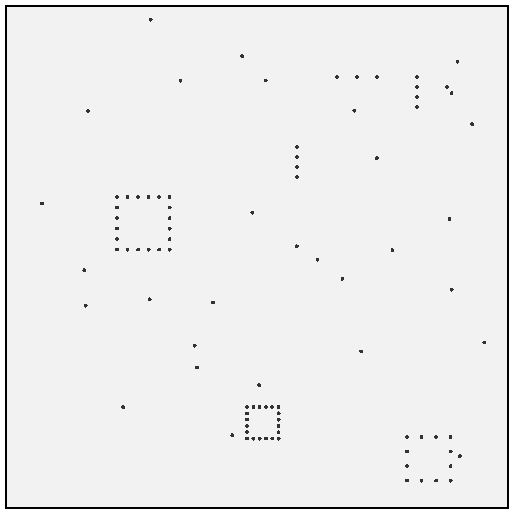
\includegraphics[width=0.44\textwidth]{img/fb100}
		\caption{Random fake PCB with 60 and 100 nodes}
		\label{fig:fakeBoards}
	\end{figure}

\newpage
\subsection{Results Exact Method}
	\begin{table}[h]
		\centering
		\begin{tabular}{lrrr}
			\toprule
			\textbf{Instance} & \textbf{Obj. Value} & \textbf{User Time (sec)} & \textbf{CPU time (sec)} \\
			\midrule
			\verb|tsp12| & 66.40 & 0.085 & 0.250 \\
			\verb|tsp60| & 629.80 & 11.240 & 36.201 \\
			\verb|rnd60| & 311.97 & 8.022 & 28.002 \\
			\verb|fb60|	& 240.47 & 24.498 & 64.486 \\
			\verb|rnd80| & 348.11 & 17.765 & 56.927 \\
			\verb|fb80| & 219.37 & 95.216 & 256.200 \\
			\verb|rnd100| & 370.09 & 30.247 & 86.565 \\
			\verb|rnd100_2| & 457.54 & 57.178 & 174.328 \\
			\verb|fb100| & 276.55 & 106.757 & 277.525 \\
			\bottomrule
		\end{tabular}
		\caption{\label{tab:ExactMethodResults} Results Exact method}
	\end{table}

	There isn't much to say about the exact method results. From the results (table~\ref{tab:ExactMethodResults}) we can see as expected that there is a trend where the increase of the number of nodes increase exponentially the CPU time (figure~\ref{fig:em-time}). This is not always case, in fact the time depends a lot by the instance. The case of \verb|tsp60|, \verb|rnd60| and \verb|rnd100|, 
	\verb|rnd100_2| show this.
	
	\begin{figure} [hb]
		\centering
		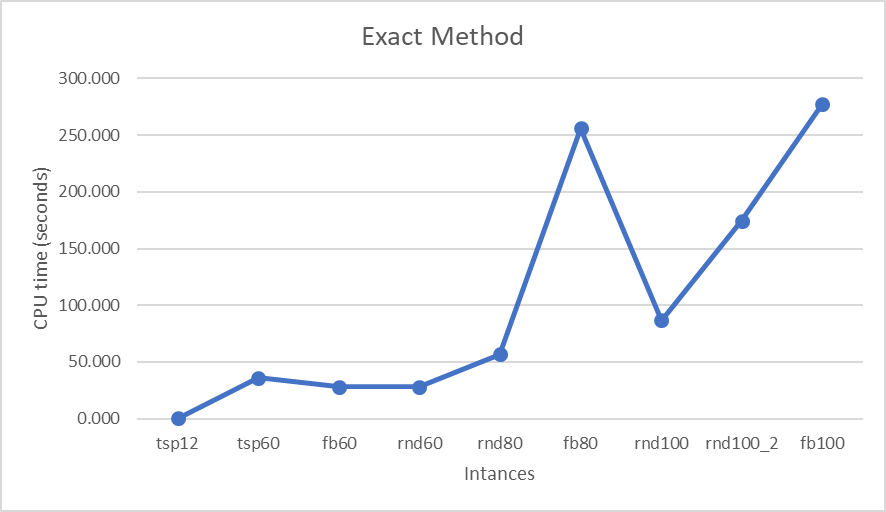
\includegraphics[width=\linewidth]{img/EM-results}
		\caption{Exact Method time for each instance}
		\label{fig:em-time}
	\end{figure}
	
	
	
\newpage
\subsection{Results Local Search}
	The Local Search is tremendously fast but at a cost of found the optimal solution only in some instance and in average it performs poorly in comparison with other methods. In this test the User time is ignore as it is equal to CPU time, no parallel computation was implemented into meta heuristics algorithm.

	It's interesting to note the average result of Local Search. I run the LS Best Improvement (BI) and LS First Improvement (FI) with 8 random initial solution for each instance. The average results show that FI is almost always the better choice at a cost of a bit more time, that is the time needed to explore more solutions.
	
	The \textbf{best strategy} for use Local Search is to start from a lot of different initial solution, in the table~\ref{tab:LS-BestStrategyResult} I summarized the results of this strategy, every local search is started with eight different random solution and the \textbf{best value} found is selected. The \textbf{CPU time} corresponds to the sum of the time of all tabu searches ran for each instance.
	
	\vspace{10pt}
	
	\begin{figure}[hb]
		\centering
		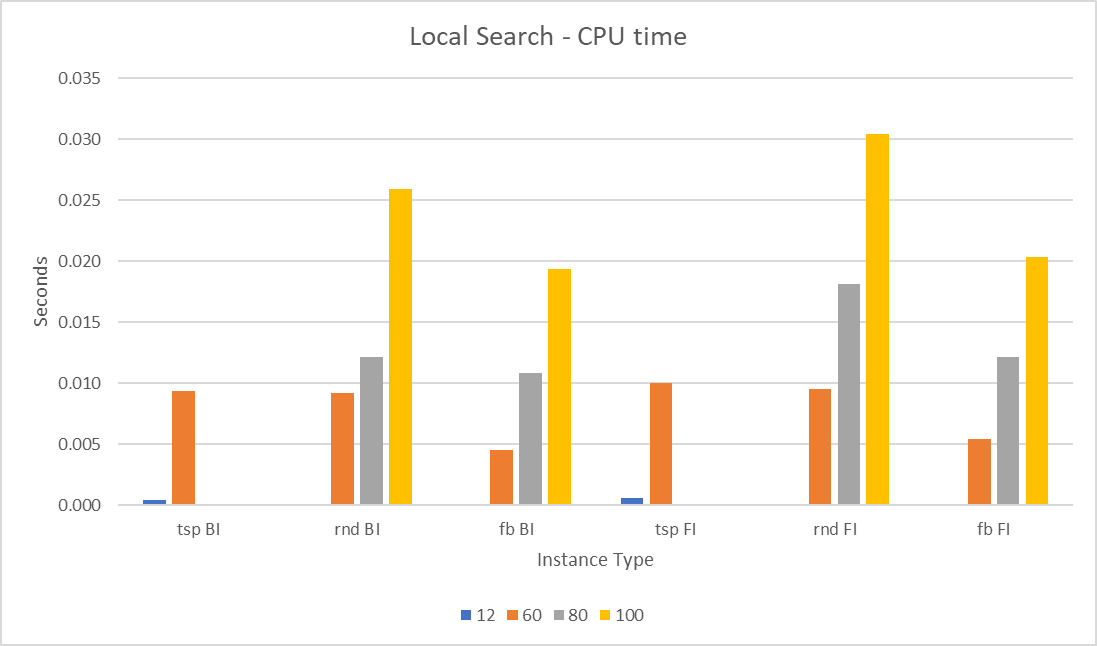
\includegraphics[width=\linewidth]{img/LS-time}
		\caption{Local Search time for each instance for each feature (BI or FI)}
		\label{fig:ls-time}
	\end{figure}
	
	
	\begin{table}
		
		\begin{tabular}{llrrr}
			\toprule
			\textbf{Instance} & \textbf{Features} & \textbf{Avg Value} & \textbf{Avg Time (s)} & \textbf{Avg Quality} (\%) \\
			\midrule
			\verb|tsp12| 	& Best Improv. & 66.850 & 4.125e-05 & 98.3 \\
			& First Improv. & 67.325 & 7.3875e-05 & 98.6 \\
			\midrule
			\verb|tsp60| 	& Best Improv. & 666.650 & 0.00071163 & 94.5 \\
			& First Improv. & 657.362 & 0.00101625 & 95.8 \\
			\midrule
			\verb|rnd60| 	& Best Improv. & 332.826 & 0.00073738 & 93.7 \\
							& First Improv. & 329.934 & 0.00096238 & 94.6 \\
			\midrule
			\verb|fb60|		& Best Improv. & 255.999 & 0.00056363 & 93.9 \\
							& First Improv. & 256.786 & 0.00067400 & 93.6 \\ 
			\midrule
			\verb|rnd80| 	& Best Improv. & 374.400 & 0.00129013 & 93.0 \\
							& First Improv. & 371.325 & 0.00198488 & 93.7 \\
			\midrule
			\verb|fb80|		& Best Improv. & 228.525 & 0.00135700 & 95.9 \\
							& First Improv. & 233.497 & 0.00151600 &  93.9 \\
			\midrule
			\verb|rnd100| 	& Best Improv. & 406.499 & 0.00266875 & 91.0 \\
							& First Improv. & 391.406 & 0.00358875 & 94.6 \\
			\midrule
			\verb|rnd100_2| & Best Improv. & 495.690 & 0.00230150 & 92.3 \\
							& First Improv. & 492.135 & 0.00302388 & 93.0 \\
			\midrule
			\verb|fb100| & Best Improv. & 296.774 & 0.00242475 & 93.2 \\
						& First Improv. & 291.699 & 0.00254362 & 95.1 \\
			\bottomrule
		\end{tabular}
		\caption{\label{tab:AvgResultLS}Average results of all Local Search BI and FI executed}
	\end{table}
	
	\begin{table}
		\centering
		\begin{tabular}{llrrr}
			\toprule
			\textbf{Instance} & \textbf{Features} & \textbf{Best Value} & \textbf{Tot. Time (s)} & \textbf{Quality (\%)} \\
			\midrule
			\verb|tsp12| & Best Improv. & 66.4 & 0.000415 & 100 \\
							& First Improv. & 66.4 & 0.000610 & 100 \\
			\midrule
			\verb|tsp60| 	& Best Improv. & 634.6 & 0.009326 & 99.2 \\
							& First Improv. & 638.6 & 0.009972 & 98.6 \\
			\midrule
			\verb|fb60|		& Best Improv. & 243.74 & 0.004509 & 98.6 \\
							& First Improv. & 243.47 & 0.005392 & 98.8 \\ 
			\midrule
			\verb|rnd60| 	& Best Improv. & 319.35 & 0.009223 & 97.7 \\
							& First Improv. & 314.53 & 0.009503 & 99.2 \\
			\midrule
			\verb|rnd80| 	& Best Improv. & 351.69 & 0.012120 & 99.0 \\
							& First Improv. & 351.05 & 0.018155 & 99.1 \\
			\midrule
			\verb|fb80| 	& Best Improv. & 223.9 & 0.010856 & 97.9 \\
							& First Improv. & 224.35 & 0.012128 & 97.7 \\
			\midrule
			\verb|rnd100| 	& Best Improv. & 387.45 & 0.028099 & 95.5 \\
							& First Improv. & 372.25 & 0.033198 & 99.4 \\
			\midrule
			\verb|rnd100_2| & Best Improv. & 476.34 & 0.023825 & 96.1 \\
							& First Improv. & 483.14 & 0.027648 & 94.7 \\
			\midrule
			\verb|fb100| & Best Improv. & 280.37 & 0.019398 & 98.6 \\
						& First Improv. & 282.99 & 0.020349 & 97.7 \\
			\bottomrule
		\end{tabular}
		\caption{\label{tab:LS-BestStrategyResult} Results of Local Search with Best Improvement and First Improvement, the result selected are only the best found from eight random initial solution}
	\end{table}
	
\newpage
\subsection{Results Tabu Search}


\subsection{Comparisons of results}

	The time of Local search is not comparable to the Exact Method.